\documentclass[11pt]{article}
\usepackage[margin=0.82in]{geometry}
\usepackage{amsmath,amssymb,booktabs,graphicx,longtable,array}
\usepackage[hidelinks]{hyperref}
\usepackage{xcolor}
\setlength{\parindent}{0pt}
\setlength{\parskip}{0.55em}
\newcommand{\fail}{\textcolor{red!70!black}{\textbf{FAIL}}}
\newcommand{\na}{\textemdash}

\title{Audit of a Five-Dimensional KDE for the\\
$n=3$ Finite-Time Total-Entropy Fluctuation Theorem}
\author{Numerical validation report}
\date{2 September 2026}

\begin{document}
\maketitle

\section*{Verdict}

The frozen five-dimensional KDE does \emph{not} resolve a reliable finite-time
total-entropy fluctuation-theorem (FT) test for the driven $n=3$ chain at
$(T_L,T_R)=(10,2)$ and block time $t=20$.  This is a negative result about the
density-estimation route, not evidence that the physical FT is false.

The conclusion follows before inspecting any total-entropy slope: the KDE
fails the exact equilibrium Gibbs-density accuracy gate at both $T=6$ and
$T=10$, two independent driven KDEs disagree beyond every frozen tolerance,
and 42 driven endpoint pairs have zero density under the frozen binned kernel.
Under the predeclared no-extrapolation rule, total-entropy sign counts, the DFT
slope, and the integral FT (IFT) were therefore not computed.

\section{Data and immutable protocol}

All samples use the projection-free Cartesian sampler with $n=3$,
$\gamma=0.1$, $\Delta t=5\times10^{-4}$, burn-in 500, block length 20,
128 independent streams, and 7813 nonoverlapping blocks per stream.  Each case
contains 1,000,064 blocks.  The driven seed is 2026083133; equilibrium seeds
are 2026090106 ($T=6$) and 2026090110 ($T=10$).

The offloaded driven CSV was deterministically restored with the original
source and seed.  Its decompressed SHA-256 is
\begin{center}
\ttfamily\small
4f728b3d0e007d704d90734b0888c00ec05b60f09385c6cfd079f3417d7a088f,
\end{center}
exactly matching the accepted original sample.  Hence this audit did not
replace the driven data with a statistically different run.

\section{KDE construction}

The reduced state is
\[
x=(I_1,I_2,I_3,\theta_1,\theta_3),
\qquad
z=(\log I_1,\log I_2,\log I_3,\theta_1,\theta_3).
\]
The estimator is a product Gaussian KDE binned on a
$48^3\times32^2$ grid.  The action axes use ordinary Gaussian convolution;
the angles use wrapped Gaussian convolution on $[-\pi,\pi)$.  The density with
respect to the physical reduced measure includes the transformation Jacobian,
\[
\log\rho_x=\log\rho_z-\sum_{j=1}^3\log I_j.
\]

Whole streams, not individual blocks, define two cross-fitting folds.  Each
endpoint is evaluated by a KDE trained only on the opposite stream fold.
Scott's five-dimensional factor uses the correlation-adjusted effective size
$N_{\rm eff}=N/g$, where $g$ is the largest initial-positive-sequence
statistical inefficiency among the three log actions and the sine/cosine of
both angles.  Here $g$ lies between 1.000 and 1.016 for the primary folds, so
$N_{\rm eff}\simeq(4.92$--$4.98)\times10^5$.  Representative action
bandwidths are 0.294--0.316 for the driven sample and 0.296--0.300 at
equilibrium; angular bandwidths are 0.398--0.423 radians.  No bandwidth
multiplier or FT fit window was tuned.

For each supported block,
\[
\Delta s_{\rm sys}=-\log\rho_x(x_{\rm end})+\log\rho_x(x_{\rm start}),
\qquad
\Delta s_{\rm tot}=\Sigma^m+\Delta s_{\rm sys}.
\]

\section{KDE accuracy: exact equilibrium test}

This section is reported before any driven FT number.  At equilibrium,
$\log\rho_{\rm exact}=-E/T+\text{constant}$ and therefore
\[
\Delta s_{\rm sys}^{\rm exact}=\frac{E_{\rm end}-E_{\rm start}}{T}.
\]
Table~\ref{tab:kde-gate} compares held-out KDE errors with thresholds frozen
before the analysis.  Unsupported points are omitted from the numerical RMSE
but reported explicitly; their presence itself forces failure.

\begin{table}[ht]
\centering
\caption{Equilibrium known-answer KDE gate.  The four frozen maxima were
0.15, 0.10, 0.25, and 0.50, respectively.}
\label{tab:kde-gate}
\small
\begin{tabular}{lrrrrr c}
\toprule
case & unsupported & endpoint & increment & tail 1\% & increment & gate\\
 & /1,000,064 & RMSE & RMSE & RMSE & $q_{.99}|e|$ & \\
\midrule
$T=6$  & 52 & 0.273456 & 0.387016 & 1.70194 & 1.38458 & \fail\\
$T=10$ & 62 & 0.270944 & 0.383225 & 1.72094 & 1.38283 & \fail\\
\bottomrule
\end{tabular}
\end{table}

Every primary error is well above its tolerance.  The increment RMSE grows
from 0.2982 ($T=6$) and 0.2925 ($T=10$) in the lowest-energy 80\% to 1.7019
and 1.7209 in the lowest-density one percent.  The tail error is therefore not
a small uniform normalization offset; it directly affects the endpoint
log-density ratios required by total entropy.

\begin{figure}[ht]
\centering
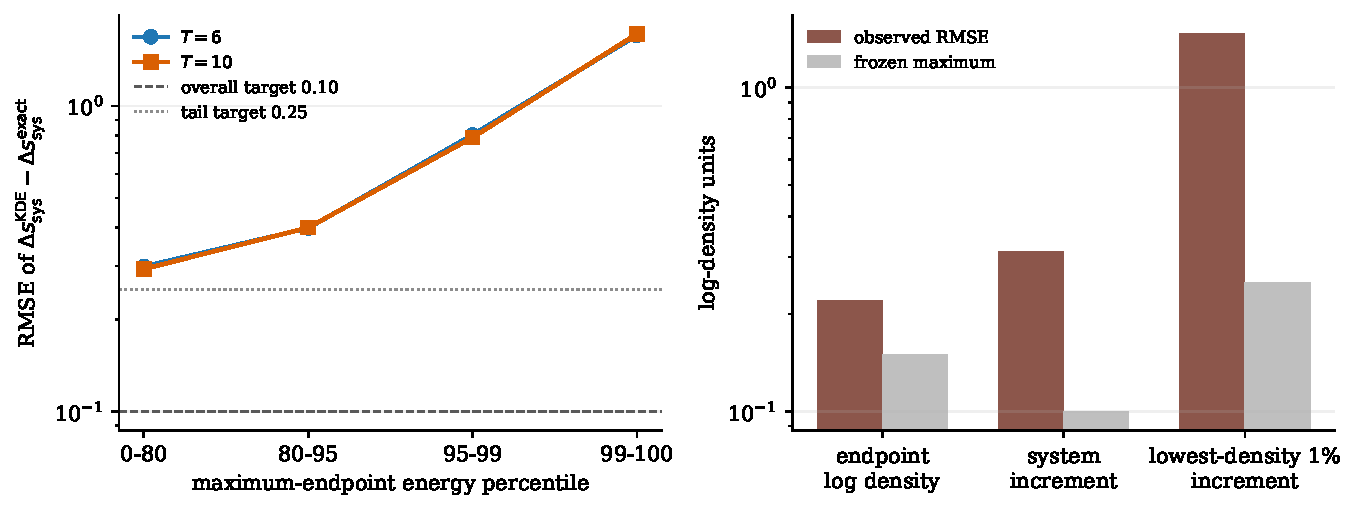
\includegraphics[width=\textwidth]{figures/kde_accuracy_audit.pdf}
\caption{Left: equilibrium system-entropy increment error grows strongly into
the low-density tail.  Right: disagreement between two independently trained
KDEs on the same held-out driven blocks also exceeds the frozen limits.}
\end{figure}

\section{Driven KDE stability and support}

Two additional KDEs were trained on disjoint stream groups and evaluated on
the same 328,146 driven audit blocks.  Twenty-six blocks lack common support.
On the 328,120 supported blocks, the centered endpoint log-density RMSE between
the two estimators is 0.220699 (limit 0.15), the system-entropy increment
disagreement RMSE is 0.311976 (limit 0.10), and the latter rises to 1.46711 in
the lowest-density one percent (limit 0.25).  Its 99th absolute percentile is
1.00570 (limit 0.50).  Thus the independent-estimator gate also fails.

In the primary two-fold fit, 1,000,022 of 1,000,064 endpoint pairs are
supported and 42 are unsupported.  On the supported subset only, the estimated
$\Delta s_{\rm sys}$ has mean $-9.09\times10^{-6}$, standard deviation 1.66178,
range $[-24.1348,26.8440]$, and one/99-percentiles $[-4.07981,4.08584]$.
These values are descriptive: removing the 42 unsupported tail blocks would
bias exactly the rare-event statistics needed for the FT.

\section{What can be reported from the driven sample}

\subsection*{Medium entropy, which does not use the KDE}

There are 41 negative medium-entropy blocks among 1,000,064:
\[
\widehat P(\Sigma^m<0)=4.0997376\times10^{-5},
\qquad
95\%\ \text{stream-bootstrap CI}
=[2.8998144,5.3996544]\times10^{-5}.
\]
The frozen Freedman--Diaconis bin width is 0.47850865.  No symmetric bin pair
has 20 observations on both sides, so no medium-entropy symmetry slope is
available.  Table~\ref{tab:raw-medium} lists every bin containing at least one
negative observation; these raw counts sum to 41.

\begin{longtable}{rrrrr}
\caption{Raw medium-entropy symmetric-bin counts with $N(-a)>0$.}
\label{tab:raw-medium}\\
\toprule
bin & $a$ interval & center & $N(+a)$ & $N(-a)$\\
\midrule
\endfirsthead
\toprule
bin & $a$ interval & center & $N(+a)$ & $N(-a)$\\
\midrule
\endhead
0  & $[0,0.4785)$       & 0.2393 & 9   & 13\\
1  & $[0.4785,0.9570)$  & 0.7178 & 13  & 4\\
2  & $[0.9570,1.4355)$  & 1.1963 & 12  & 3\\
3  & $[1.4355,1.9140)$  & 1.6748 & 8   & 6\\
4  & $[1.9140,2.3925)$  & 2.1533 & 21  & 7\\
5  & $[2.3925,2.8711)$  & 2.6318 & 38  & 1\\
6  & $[2.8711,3.3496)$  & 3.1103 & 39  & 2\\
8  & $[3.8281,4.3066)$  & 4.0673 & 69  & 2\\
10 & $[4.7851,5.2636)$  & 5.0243 & 81  & 1\\
13 & $[6.2206,6.6991)$  & 6.4599 & 121 & 1\\
15 & $[7.1776,7.6561)$  & 7.4169 & 151 & 1\\
\bottomrule
\end{longtable}

\begin{figure}[ht]
\centering
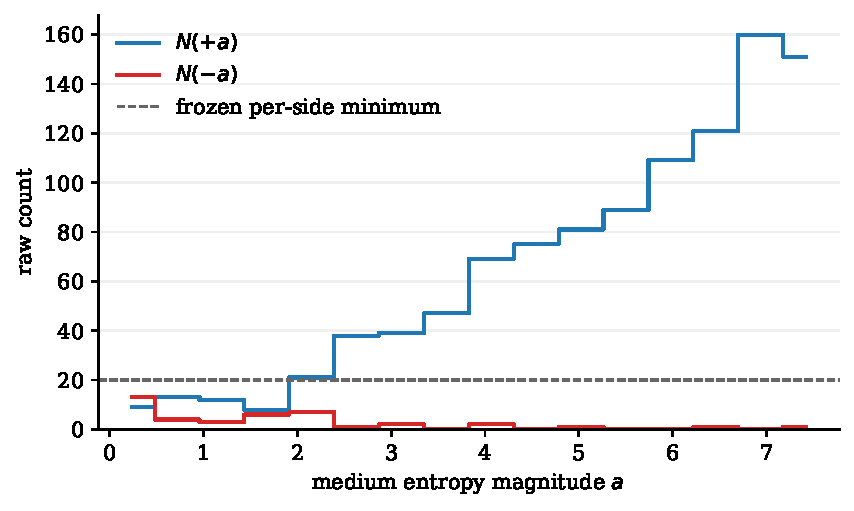
\includegraphics[width=0.72\textwidth]{figures/medium_entropy_raw_support.pdf}
\caption{Raw two-sided medium-entropy support.  Neither side reaches the
predeclared minimum of 20 in the same bin.}
\end{figure}

The medium-only exponential diagnostic is also unresolved:
\[
\log\langle e^{-\Sigma^m}\rangle=-5.7735605,
\qquad 95\%\ \text{CI}=[-8.0873157,-4.8624448].
\]
Its exponential-weight effective sample size is only 2.2880 out of 1,000,064;
one block contributes 61.55\% of the sum and deleting one stream can change the
log average by 0.9481.  This number is not a resolved IFT test, and medium
entropy is not the exact finite-time total entropy.

\subsection*{Total entropy}

The total-entropy entries are intentionally recorded as ``not computed'':

\begin{center}
\begin{tabular}{lc}
\toprule
quantity & result\\
\midrule
$\#\{\Delta s_{\rm tot}<0\}$ & not computed (42 unsupported pairs)\\
$P(\Delta s_{\rm tot}<0)$ & not computed\\
DFT slope and confidence interval & not computed\\
$\log\langle e^{-\Delta s_{\rm tot}}\rangle$ & not computed\\
\bottomrule
\end{tabular}
\end{center}

Filling these points with a density floor, an infinite-kernel tail, or
plus-four pseudo-counts would manufacture precisely the negative-tail evidence
the audit is designed to test.

\section{Integrity and provenance}

All three input archives pass Zstandard integrity checks and their
decompressed hashes match the predeclared values.  Every archive contains
1,000,064 ordered finite rows; consecutive saved endpoints agree exactly at
output precision.  The driven identity
$\Sigma^m=-Q_L/10-Q_R/2$ has maximum absolute recomputation error
$2.84217\times10^{-14}$.  The restored simulator reports zero midpoint
failures and first-law residual RMS rate $1.48691\times10^{-5}$.

\resizebox{\textwidth}{!}{%
\begin{tabular}{@{}ll@{}}
\toprule
item & SHA-256 / identifier\\
\midrule
frozen scientific protocol & commit \texttt{0b53e573afdd324fa44b4c7cb50c8bc579d40838}\\
unsupported-point handling & commit \texttt{0faec919ad58ca8504a6d08a660f1c3492feadfc}\\
CSV implementation fix & commit \texttt{4e423a965ae076039f7aa3b37fac8b3842b93b1f}\\
simulator source & \texttt{9ae5835ed708c8794c8b00ba799b23761482953aaf0ed47cd0b4ba3966d4eaf2}\\
simulator binary & \texttt{93c4aa6d046f3c35cd0ea1136091fc44ef1b64baf6237e4663ca9e86b995a156}\\
analysis source & \texttt{59ddfdb9d530116be169a9ce2651b44580f9c7cc666c7a4f4435e9728dc80e7c}\\
driven compressed data & \texttt{5979d35dd335574bc01add81d4c8d97759151a62f4fd6acadc111eb6bdccd7a2}\\
\bottomrule
\end{tabular}%
}

The exact restoration command was
\begin{verbatim}
entropy_ft_n3_eq sample_n3 10 2 3 8 500 20 7813 0.0005 \
  2026083133 8 raw/driven 1
\end{verbatim}
and the final analysis command was
\begin{verbatim}
python3 analyze_kde_ft.py --driven raw/driven_blocks.csv.zst \
  --equilibrium-t6 ../entropy_ft_n3_equilibrium_2026-09-01/raw/T6_blocks.csv.zst \
  --equilibrium-t10 ../entropy_ft_n3_equilibrium_2026-09-01/raw/T10_blocks.csv.zst \
  --output analysis
\end{verbatim}

\section*{Claim boundary}

This experiment establishes that the specified cross-fitted five-dimensional
KDE is insufficiently accurate in the endpoint tails to extend the exact
finite-time total-entropy FT from $n=2$ to $n=3$.  It neither validates nor
falsifies the physical $n=3$ FT.  A future total-entropy claim requires a
stationary-density or density-ratio estimator that passes the exact Gibbs
tail audit and yields nonzero, stable support for every driven endpoint used in
the two-tail statistic.

\end{document}
